\section{Introduction}

\begin{wrapfigure}[18]{r}{0.5\textwidth}
   \vspace{-45pt}
   \centering
   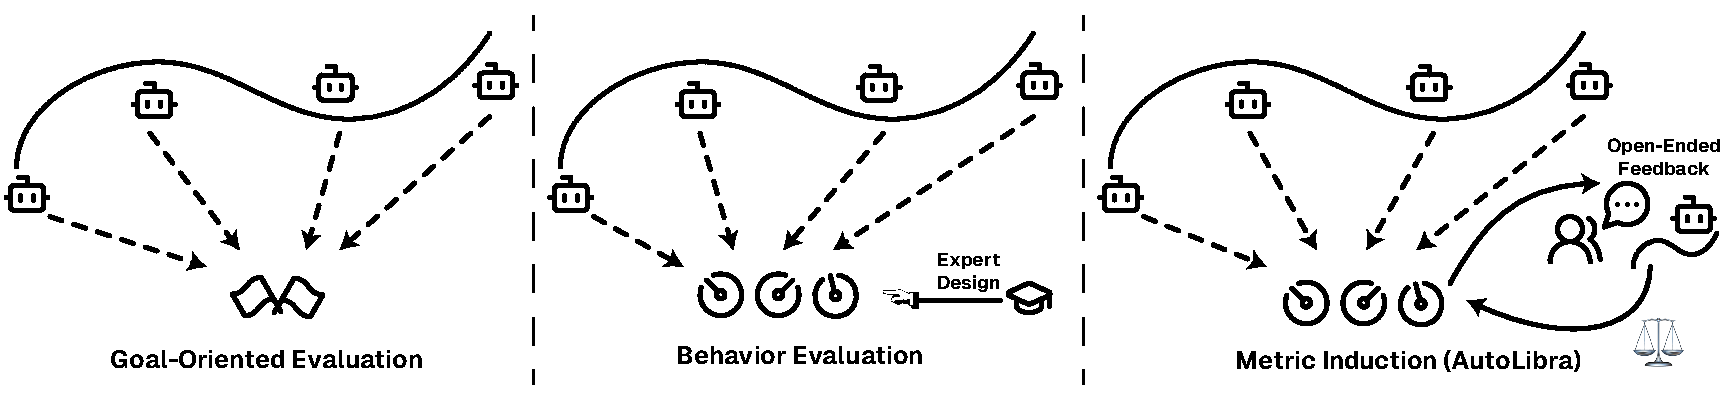
\includegraphics[width=0.5\textwidth]{figs/autolibra.pdf}
   \caption{Comparison of AutoLibra with existing agent evaluation paradigms.}
\end{wrapfigure}


Feedback is critical for human self-assessment and improvement \citep{nicol2006formative}.

Compared to the scarce reward
we get from achieving goals, these metrics offer a lens for self-reflection on the
strengths and weaknesses of ourselves and a ladder for self-improvement.
In this paper, we ask:
\textbf{can we automatically induce metrics to evaluate and improve language agents from natural language feedback?} 

   
The current evaluation of large language model (LLM) agents and reward modeling often fall
into two paradigms: (1) goal-oriented evaluation --
\emph{whether the agents have fulfilled the given task},
\emph{e.g.} \citet{zhouwebarena,jimenezswe,chan2024mle,paglieri2024balrog}
and (2) behavior evaluation -- \emph{how well the agents do on heuristically designed dimensions},
\emph{e.g.} \citet{zhousotopia,shao2024collaborative,pan2025why}. 
Goal-oriented evaluation is often verifiable, but it is not fine-grained or comprehensive enough
to diagnose agents' behavior problems or find the bottlenecks for improvements. 
While behavior evaluation complements it, it requires manual design of the metrics by experts,
which is time-consuming, may not align with users' opinions, and often not concrete enough. 

We introduce AutoLibra \protect\includegraphics[height=1em]{figs/scale.png}, an automatic metric induction method,
as a new paradigm for agent evaluation and improvement.
This method offers behavior evaluation for agents, while (1) automating the metric creation process with LLMs, 
(2) optimizing the alignment through searching for a set of metrics to cover human feedback with minimal redundancy,
and (3) providing concrete examples of good and bad behaviors for each metric to improve the
LLM-as-a-Judge's performance. 

AutoLibra takes in agent trajectories along with human open-ended feedback, and generates a set of metrics, each with a name, description, and a list of good behavior examples, and bad behavior examples. AutoLibra 



\begin{wrapfigure}{r}{0.7\textwidth}
    \centering
    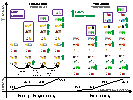
\includegraphics[width=0.7\textwidth]{figs/autolibra-teaser.pdf}
    \caption{Caption}
    \label{fig:enter-label}
\end{wrapfigure}